\documentclass{beamer}
\usepackage[utf8]{inputenc}

\usetheme{Madrid}
\usecolortheme{default}
\usepackage{amsmath,amssymb,amsfonts,amsthm}
\usepackage{txfonts}
\usepackage{tkz-euclide}
\usepackage{listings}
\usepackage{adjustbox}
\usepackage{array}
\usepackage{tabularx}
\usepackage{gvv}
\usepackage{lmodern}
\usepackage{circuitikz}
\usepackage{tikz}
\usepackage{graphicx}

\setbeamertemplate{page number in head/foot}[totalframenumber]

\usepackage{tcolorbox}
\tcbuselibrary{minted,breakable,xparse,skins}



\definecolor{bg}{gray}{0.95}
\DeclareTCBListing{mintedbox}{O{}m!O{}}{%
  breakable=true,
  listing engine=minted,
  listing only,
  minted language=#2,
  minted style=default,
  minted options={%
    linenos,
    gobble=0,
    breaklines=true,
    breakafter=,,
    fontsize=\small,
    numbersep=8pt,
    #1},
  boxsep=0pt,
  left skip=0pt,
  right skip=0pt,
  left=25pt,
  right=0pt,
  top=3pt,
  bottom=3pt,
  arc=5pt,
  leftrule=0pt,
  rightrule=0pt,
  bottomrule=2pt,
  toprule=2pt,
  colback=bg,
  colframe=orange!70,
  enhanced,
  overlay={%
    \begin{tcbclipinterior}
    \fill[orange!20!white] (frame.south west) rectangle ([xshift=20pt]frame.north west);
    \end{tcbclipinterior}},
  #3,
}
\lstset{
    language=C,
    basicstyle=\ttfamily\small,
    keywordstyle=\color{blue},
    stringstyle=\color{orange},
    commentstyle=\color{green!60!black},
    numbers=left,
    numberstyle=\tiny\color{gray},
    breaklines=true,
    showstringspaces=false,
}
%------------------------------------------------------------

\title
{3.4.3}
\author 
{AI25BTECH11034 - Sujal Chauhan }



\begin{document}

\frame{\titlepage}
\begin{frame}{Question}

Construct a square of side 3 unit
\end{frame}


\begin{frame}{Solution}
Let's consider four points A,B,C,D as vertices of square:
\begin{center}
    \begin{tabular}{|c|c|} \hline
       Point  & Positon Vector \\ \hline
       A  & \myvec{0 \\ 0} \\ \hline
       B  & \myvec{3 \\ 0} \\ \hline
       C  & \myvec{3\\ 3} \\ \hline
       D  & \myvec{0 \\ 3} \\ \hline
    \end{tabular}
\end{center}
\end{frame}
\begin{frame}{Figure}
\begin{figure}[h]
    \centering
    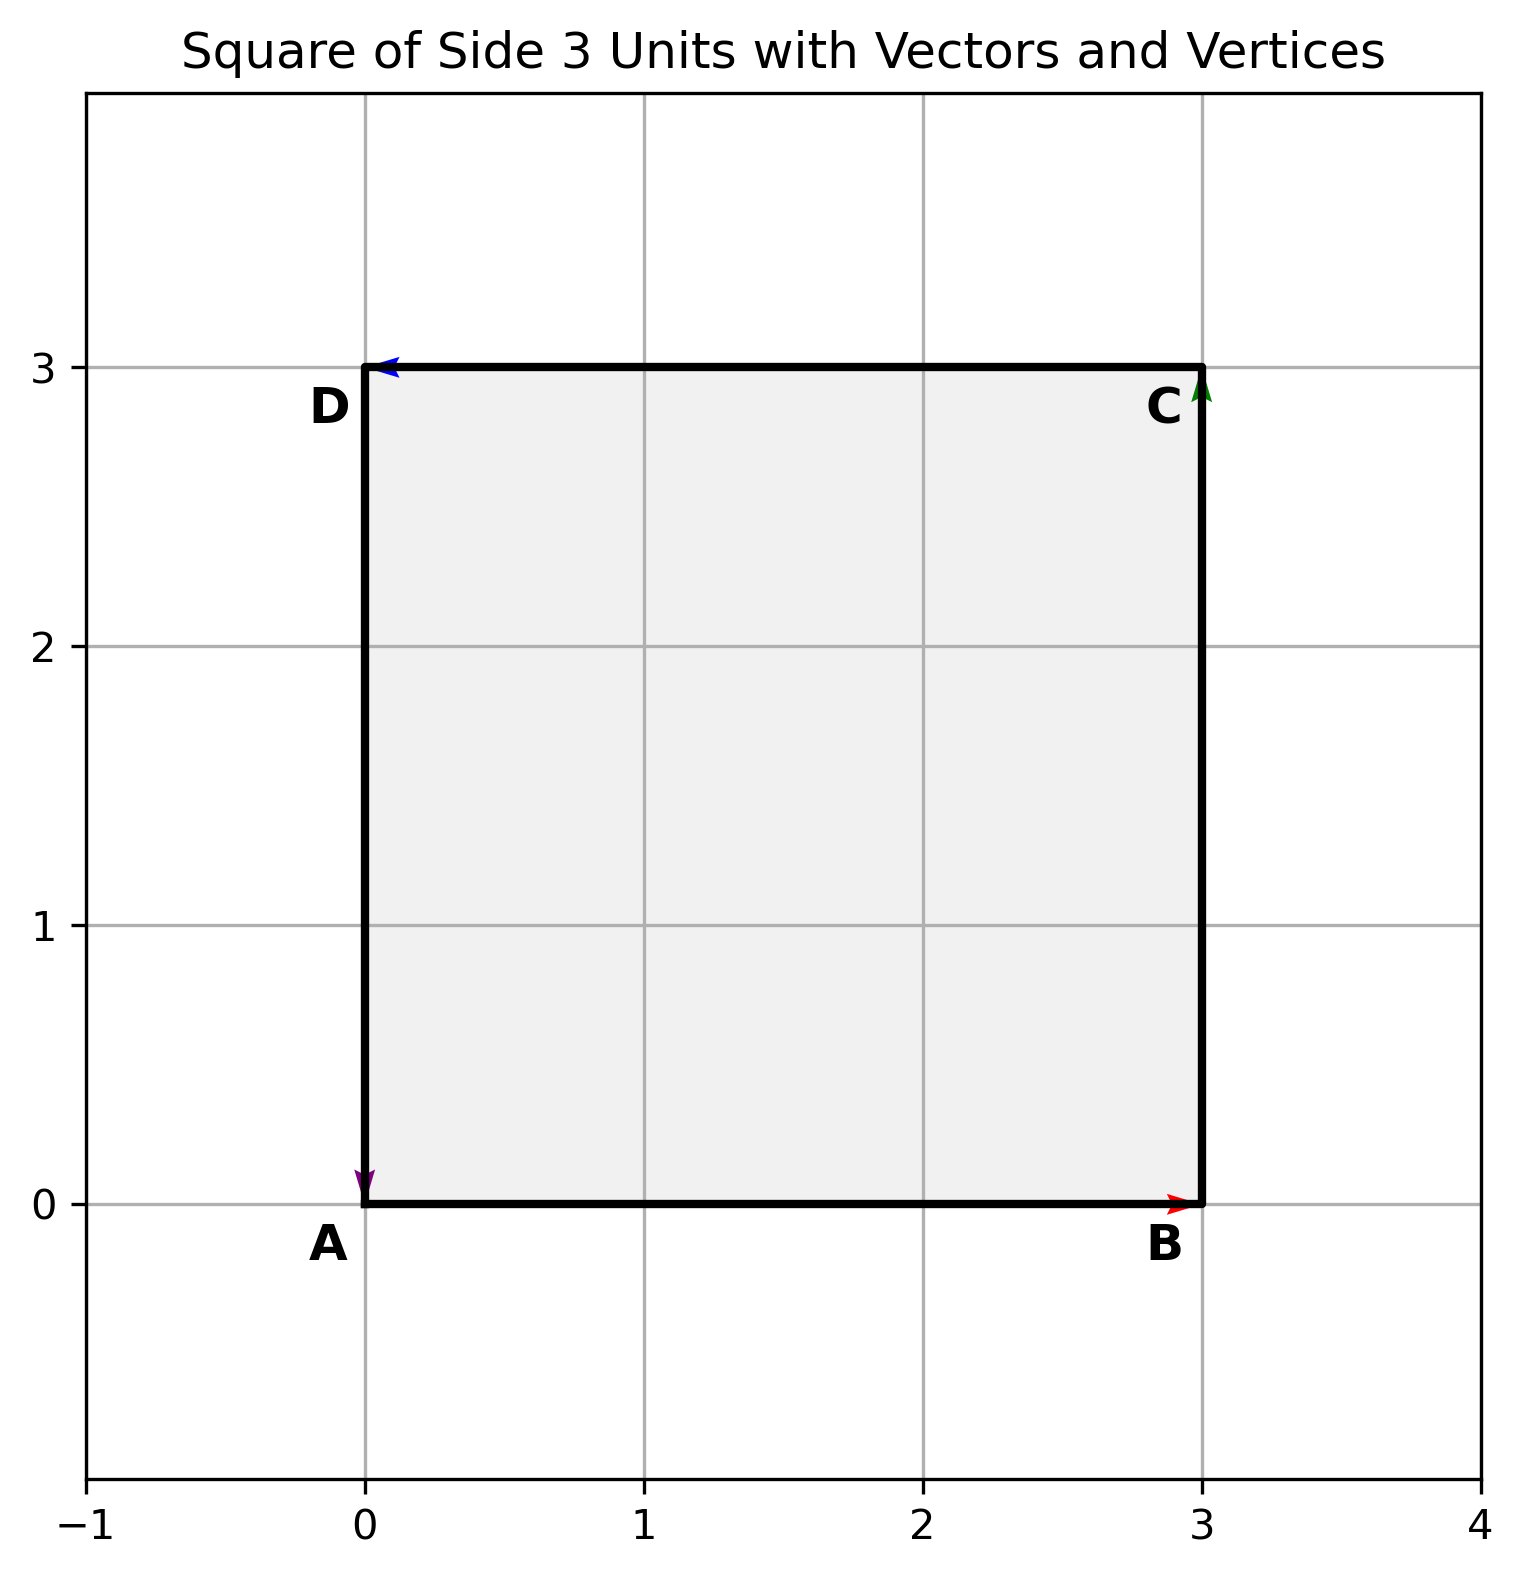
\includegraphics[width=0.5\linewidth]{figures/square_plot.png}
    \caption{Caption}
    \label{square}
\end{figure}

\end{frame}
\begin{frame}{Properties of Square}

\begin{enumerate}
    \item All sides have equal length
    \item Opposite sides are parallel
    \item Diagonals have equal length
    \item Adjecent sides are perpendicular to each other
\end{enumerate}
\end{frame}
\begin{frame}{Properties of Square}
    \begin{align}
        \norm{\Vec{A}-\Vec{B}}= \norm{\Vec{B}-\Vec{C}}= \norm{\Vec{C}-\Vec{D}}= \norm{\Vec{D}-\Vec{A}}
    \end{align}
    \begin{align}
        \Vec{A}-\Vec{B}=\Vec{D}-\Vec{C}
    \end{align}
    \begin{align}
         \norm{\Vec{A}-\Vec{C}}= \norm{\Vec{B}-\Vec{D}}
    \end{align}
    \begin{align}
        0=(\Vec{A}-\Vec{B})^T(\Vec{B}-\Vec{C})=(\Vec{B}-\Vec{C})^T(\Vec{C}-\Vec{D})=(\Vec{C}-\Vec{D})^T(\Vec{D}-\Vec{A})=(\Vec{D}-\Vec{A})^T(\Vec{A}-\Vec{B})
\end{align}



\end{frame}
\end{document}
